\documentclass[cal1spr16Lectures.tex]{subfiles}

\begin{document}

%\section[Week 9]{Week 9: 14-18 Mar}

% % % 
\subsubsection{\bf Wednesday 16 March}
% % %

\begin{frame}[allowframebreaks]{Wed 16 Mar}
\begin{itemize}\footnotesize
\item Midterm: Take your raw score out of 140, instead of 150, for the curve.

\begin{center}
\includegraphics[scale=0.4]{..//MidtermSpread}
\end{center}

\item Office hours 1030-1230 today and Friday.
\end{itemize}
\end{frame}

% % %
\subsection[4.1 Maxima and Minima]{\S 4.1 Maxima and Minima}
% % %

% % %
\begin{frame}{\S 4.1 Maxima and Minima}
Chapter 4 is all about applications of the derivative.  In the first couple of sections we examine the graphs of functions and what the derivative can tell us about the graph's behavior and characteristics.
\end{frame}

% % %
\begin{frame}
\small 
\begin{dfn} Let $f$ be defined on an interval $I$ containing $c$.
\begin{itemize}
\item $f$ has an {\bf absolute maximum} value on $I$ at $c$ means $f(c)\ge f(x)$ for every $x$ in $I$.
\item $f$ has an {\bf absolute minimum} value on $I$ at $c$ means $f(c)\le f(x)$ for every $x$ in $I$.
\end{itemize}
\end{dfn}
\end{frame}

% % %
\begin{frame}
\footnotesize
The existence and location of absolute extreme values depend on the function and the interval of interest:
\begin{columns}[T]
\begin{column}{.5\textwidth}
\begin{block}{}
\centering{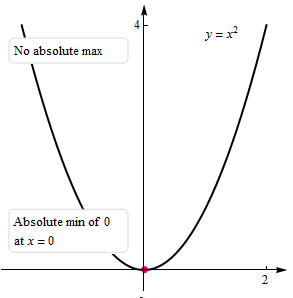
\includegraphics[scale=0.65]{pictures/Fig4_2a}}
\end{block}
\end{column}
\begin{column}{.5\textwidth}
\begin{block}{}
\centering{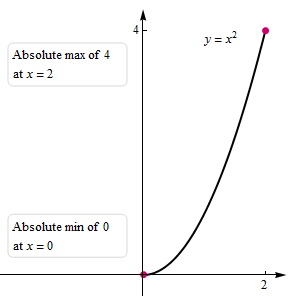
\includegraphics[scale=0.65]{pictures/Fig4_2b}}
\end{block}
\end{column}
\end{columns}
\end{frame}

% % %
\begin{frame}
\frametitle{}
\begin{columns}%[T]
\begin{column}{.5\textwidth}
\begin{block}{}
\centering{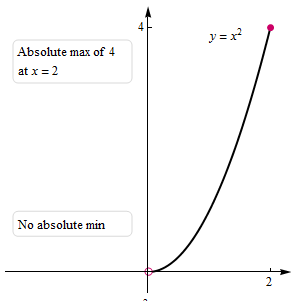
\includegraphics[scale=0.65]{pictures/Fig4_2c}}
\end{block}
\end{column}
\begin{column}{.5\textwidth}
\begin{block}{}
\centering{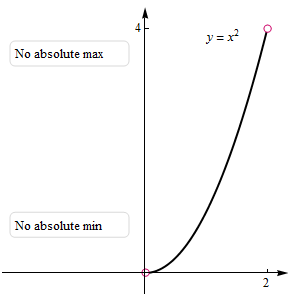
\includegraphics[scale=0.65]{pictures/Fig4_2d}}
\end{block}
\end{column}
\end{columns}
\end{frame}

% % %
\subsubsection{Extreme Value Theorem}
% % % 

% % %
\begin{frame}{\small Extreme Value Theorem}
\small
\begin{thm}[Extreme Value Theorem] A function that is continuous on a closed interval $[a,b]$ has an absolute maximum value and an absolute minimum value on that interval. \end{thm}

\vspace{1pc}
The EVT provides the criteria that ensures absolute extrema:
\begin{itemize}
\item the function must be continuous on the interval of interest;
\item the interval of interest must be closed and bounded.
\end{itemize}
\end{frame}

% % %
\subsubsection{Local Maxima and Minima}
% % %

% % %
\begin{frame}{\small Local Maxima and Minima}
\small
Beyond absolute extrema, a graph may have a number of peaks and dips throughout its interval of interest:
\begin{center}
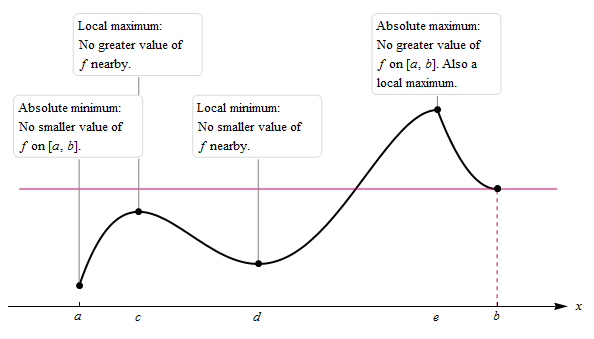
\includegraphics[scale=0.625]{pictures/Fig4_5}
\end{center}
\end{frame}

% % %
\begin{frame}
\frametitle{}
\small
\begin{dfn} Suppose $I$ is an interval on which $f$ is defined and $c$ is an interior point of $I$.
\begin{itemize}
\item If $f(c)\ge f(x)$ for all $x$ in some open interval containing $c$, then $f(c)$ is a {\bf local maximum} value of $f$.
\item If $f(c)\le f(x)$ for all $x$ in some open interval containing $c$, then $f(c)$ is a {\bf local minimum} value of $f$.
\end{itemize}
\end{dfn}
\end{frame}

% % %
\begin{frame}
\frametitle{}
\small
\begin{exe} Use the graph below to identify the points on the interval $[a,b]$ at which local and absolute extreme values occur.
\begin{center}
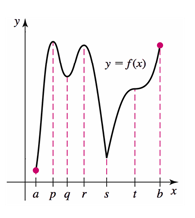
\includegraphics[scale=0.9]{pictures/Ch4Sect1_Prob16}
\end{center}
\end{exe}
\end{frame}

% % %
\subsubsection{Critical Points}
% % %

% % %
\begin{frame}{\small Critical Points}
Based on the previous graph, how is the derivative related to where the local extrema occur?

\vspace{1pc}
Local extrema occur where the derivative either does not exist or is equal to 0.

\begin{dfn} An interior point $c$ of the domain of $f$ at which $f^{\prime}(c)=0$ or $f^{\prime}(c)$ fails to exist is called a {\bf critical point} of $f$. \end{dfn}
\end{frame}

% % %
\subsubsection{Local Extreme Point Theorem}
% % %

% % %
\begin{frame}{\small Local Extreme Point Theorem}
\small
\begin{thm}[Local Extreme Point Theorem] If $f$ has a local minimum or maximum value at $c$ and $f^{\prime}(c)$ exists, then $f^{\prime}(c)=0$.  \alert{\bf (Converse is not true!)} \end{thm}

It is possible for $f^{\prime}(c)=0$ or $f^{\prime}(c)$ not to exist at a point, yet the point not be a local min or max.  Therefore, critical points provide {\bf candidates} for local extrema, but do not guarantee that the points are local extrema (see p.\ 227 immediately before Figure 4.9 for examples).
\end{frame}

% % %
\subsubsection{Locating Absolute Min and Max}
% % %

% % %
\begin{frame}{\small Locating Absolute Min and Max}
%\small
Two facts help us in the search for absolute extrema:

\begin{itemize}
\item Absolute extrema in the interior of an interval are also local extrema, which occur at critical points of $f$.
\item Absolute extrema may occur at the endpoints of $f$.
\end{itemize}
\end{frame}

% % %
\begin{frame}
\frametitle{}
\footnotesize
{\bf Procedure: } Assume that the function $f$ is continuous on $[a,b]$.

\begin{itemize}
\item[1.] Locate the critical points $c$ in $(a,b)$, where $f^{\prime}(c)=0$ or $f^{\prime}(c)$ does not exist.  These points are {\bf candidates} for absolute extrema.
\item[2.] Evaluate $f$ at the critical points and at the endpoints of $[a,b]$.
\item[3.] Choose the largest and smallest values of $f$ from Step 2 for the absolute max and min values, respectively.
\end{itemize}

NOTE:  In this section, given an equation, we can identify critical points and absolute extrema, \alert{BUT NOT LOCAL EXTREMA}.  Techniques for locating local extrema come in later sections.
\end{frame}

% % % 
\begin{frame}
\begin{ex}
On the interval $[-2,2]$, the function $f(x)=x^4$
\begin{itemize}
\item[A. ] has no local or absolute extrema.
\item[B. ] has a local minimum but no absolute minimum.
\item[C. ] has an absolute maximum but no local maxima.
\item[D. ] has an absolute maximum at an interior point of the interval.
\end{itemize}
\end{ex}
\end{frame}

% % %
\begin{frame}%[t]
\frametitle{}
\begin{exe} Given $f(x)=(x+1)^{4/3}$ on $[-8,8]$, determine the critical points and the absolute extreme values of $f$. \end{exe}
\end{frame}

% % %
\subsubsection{Book Problems}

% % %
\begin{frame}
\begin{block}{4.1 Book Problems}
11--35 (odds), 37--49 (odds) 
\end{block}
\end{frame}

\end{document}